\capitulo{4}{Técnicas y herramientas}

En esta sección se exponen las herramientas y bibliotecas que se han aprendido y utilizado a lo largo del desarrollo del proyecto.
A lo largo del ciclo de vida del proyecto, el proyecto experimentó varios cambios, incluyendo la sustitución o eliminación de algunas bibliotecas. Sin embargo, es importante destacar todas estas herramientas, ya que cada una ha tenido un impacto significativo en el proyecto y han sido fundamentales en diferentes etapas del mismo.

\section{Herramientas}

Se muestra a continuación las herramientas usadas a lo largo del desarrollo del proyecto.

\subsection{React Native}

La elección del \textit{framework} adecuado juega un papel crucial en el éxito de un proyecto. Dicha elección se complica aún más cuando se carece de experiencia previa en el desarrollo de aplicaciones móviles. Dentro del gran abanico de posibilidades React Native y Flutter emergen como grandes líderes en el sector gracias a sus grandes comunidades y la abundancia de recursos en línea. Por otro lado se pueden descartar directamente opciones como el entorno de desarrollo de iOS (por ejemplo, el uso de Swift y Cocoa Touch) debido a su exclusividad para aplicaciones para iOS debido a que el objetivo de este proyecto es desarrollar una aplicación para Android.

React Native se presenta como mi elección favorita. Este es un \textit{framework} de código abierto creado por Facebook orientado a la creación de aplicaciones nativas tanto en iOS como en Android. React Native está basado en JavaScript y React, una biblioteca de JavaScript destinada a la creación de interfaces de usuario. Fue lanzado en 2015 con el propósito de superar las limitaciones del desarrollo de aplicaciones móviles basado solo en HTML5, en las que simplemente se adapta aplicaciones web a un entorno móvil. React Native utiliza componentes nativos en lugar de WebViews para la interfaz de usuario, esto conlleva a que las aplicaciones se sientan y actúen como en una aplicación nativa.
Uno de los elementos más importantes de este \textit{framework} es el ´React Native Bridge' (ver imagen \ref{img:puenteRN}), el cual facilita la comunicación entre el código JavaScript y los elementos nativos del dispositivos. El ´puente' maneja de forma paralela dos flujos de trabajo, uno ejecuta la lógica de la aplicación en JavaScript y otro gestiona las operaciones de la interfaz de usuario nativa. Esto permite que las aplicaciones en React Native accedan a las características del dispositivo como la cámara o la ubicación, ofreciendo una experiencia fluida para el usuario gracias a características como el \textit{hot reload}.

\begin{figure}[h]
	\label{img:puenteRN}
	\centering
	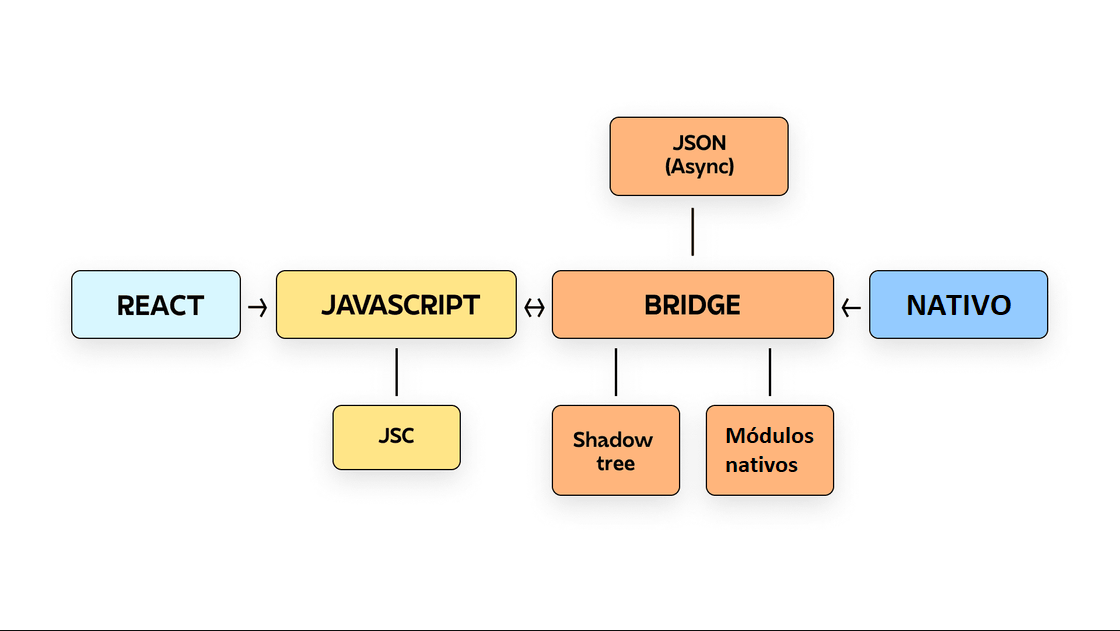
\includegraphics[width=\textwidth]{puenteRN}
	\caption[flujo trabajo React Native]{Flujo de trabajo y arquitectura de una aplicación React Native~\cite{RNarquitectura}.}
\end{figure}

Mi preferencia de este \textit{framework} sobre el resto radica en mi familiaridad previa con la programación web y JavaScript, lo cual reducirá la curva de aprendizaje en la transición hacia React Native en contraste con otros \textit{framework} que podrían requerir el aprendizaje de nuevos lenguajes de programación o paradigmas de programación. 
Por otro lado, uno de los grandes motivos de este \textit{framework} es su gran popularidad, el cual se traduce en una gran riqueza de recursos disponibles, como bibliotecas, videotutoriales o foros, cruciales a la hora de enfrentar los desafíos que puedan surgir. 
Finalmente aunque para este proyecto no sea un requerimiento hay que tener en cuenta la gran versatilidad de React Native, el cual permite la creación de aplicaciones nativas tanto en Android como en iOS a partir de un único código base. Optimizando así el proceso de desarrollo permitiendo en un futuro poder dar cobertura a un mercado más amplio sin esfuerzos duplicados.

Como había nombrado anteriormente Flutter es otro \textit{framework} que destaca sobre el resto y ofrece ciertas ventajas notables sobre React Native, como un rendimiento superior gracias al uso de su motor de renderizado propio y la gran capacidad de personalización de la interfaz de usuario. Aunque Flutter pudiera ser superior en algunos aspectos técnicos sigo decantándome por React Native debido a su gran comunidad y la familiaridad que tengo con las tecnologías web, priorizando así un aprendizaje más sencillo frente a posibles mejoras en el rendimiento. Por otro lado existen los \textit{frameworks} Ionic y Xamarin que los he descartado debido a sus limitaciones en términos de acceso a funciones nativas y comunidades bastante inferiores comparado con React Native o Flutter. Kotlin era un opción con gran potencial para el desarrollo nativo de aplicaciones Android pero la descarté rápidamente por tener una curva de aprendizaje más pronunciada que su competencia, ya que representaría un obstáculo significativo en cuanto al tiempo de desarrollo sin garantizar beneficios proporcionales a dicho esfuerzo.

Respecto a Angular, si bien este \textit{framework} ofrece un ecosistema robusto para el desarrollo de aplicaciones web dinámicas y complejas utilizando TypeScript, es importante mencionar que también es posible desarrollar aplicaciones móviles con Angular, ofreciendo una experiencia cercana a la nativa, aunque a través de un enfoque diferente al de las aplicaciones nativas desarrolladas con React Native. 
Angular no deja de ser una elección excelente, pero debido a la preferencia del proyecto de enfocarse en una aplicación móvil sin la necesidad de dar soporte de navegador, Angular puede no ser la opción más adecuada para el proyecto.
Por lo tanto he descartado Angular buscando una solución más enfocada y optimizada para el desarrollo móvil, aprovechando las capacidades nativas de los dispositivos móviles.


\subsection{Expo}

Expo es un \textit{framework} que simplifica el desarrollo de aplicaciones móviles con React Native, actuando como una capa de abstracción reduciendo las barreras de entrada al desarrollo móvil. 
Consta de un entorno y herramientas listas para usar, eliminando la necesidad de configurar sistemas de construcción nativos complejos. 
Ofrece un conjunto de APIs disponibles a través de módulos que se pueden invocar directamente desde el código JavaScript las cuales cubren funcionalidades comunes del dispositivo, como cámara, geolocalización o notificaciones sin requerir de configuración adicional. 

Expo ha sido fundamental en el proyecto para desarrollar la interfaz de usuario permitiendo probar y visualizar cambios en tiempo real en diferentes plataformas.
Una de las funcionalidades significativas de Expo ha sido su capacidad para facilitar la ejecución y testeo de la aplicación directamente en dispositivos móviles personales sin necesidad de configurar emuladores. Esto se logra mediante el uso de la aplicación Expo Go en el teléfono móvil y escaneando un código QR generado por el entorno de desarrollo Expo.
Expo ha tenido un papel fundamental en las fases de prueba y depuración, permitiendo probar la aplicación en un entorno real y ajustar la interfaz de usuario con un ciclo de retroalimentación casi instantáneo.


\subsection{Firebase}

Firebase es una plataforma de Google creada para el desarrollo de aplicaciones móviles y web.
Cuenta con un amplio conjunto de servicios integrados que permiten crear aplicaciones robustas y de alta calidad sin necesidad de gestionar la infraestructura subyacente.

Ente el amplio abanico de servicios que ofrece, destacan los siguientes:
 
\begin{itemize}

\item \textbf{FireBase Authentication:} Provee diversos servicios de autenticación de usuarios, como inicio de sesión con correo electrónico, Google, FaceBook y Github entre otros. Facilitando la implementación de una amplia gama de servicios de autenticación sin necesidad de manejar detalles complicados de seguridad.

\item \textbf{FireStore:} Ofrece soluciones de bases de datos en tiempo real y basadas en la nube. Esto permite sincronizar datos entre los usuarios en tiempo real, a parte, FireStore ofrece una estructura fácilmente escalable.

\item \textbf{FireBase Cloud Messaging:} Sistema que permite enviar notificaciones a los usuarios de forma segura mediante correo y teléfono. Aunque para la versión gratuita este servicio es muy limitado.

\item \textbf{FireBase Analytics:} Ofrece una herramienta poderosa para analizar el uso de la aplicación por parte de los usuarios.
Permitiendo rastrear eventos específicos, obtener información demográfica de los usuarios, analizar la duración y frecuencia de las sesiones, y monitorear la retención y la ejecución de objetivos preestablecidos.

\item \textbf{FireBase Cloud Functions:} Permite ejecutar código backend en respuesta a eventos desencadenados por alguno de los servicios de Firebase.
Es de gran utilidad para ejecutar ciertas tareas en el lado del servidor, como procesamiento de pagos o el envió de correos electrónicos. 

\end{itemize}

Es una herramienta de gran potencial que se integra perfectamente con React Native a través de módulos y SDKs.
Proveyendo a los desarrolladores una variedad de herramientas preconstruidas y escalables a medida que la aplicación crece sin necesidad de ninguna intervención.


\subsection{Solidity}

Solidity es un lenguaje de programación de contratos orientado a objetos y de alto nivel diseñado específicamente para escribir \textit{smart contracts} que se ejecutan en la Ethereum Virtual Machine (EVM). Consta de una sintaxis que recuerda a lenguajes como JavaScript, C++ o Python, lo que facilita su aprendizaje. 
Es un lenguaje de tipado estático, asegurando que el tipo de cada variable se define en tiempo de compilación y no cambia durante al ejecución del contrato, aumentando así la seguridad y ayudando a la detección de errores antes de la ejecución.

Una de las características más destacadas de Solidity es su soporte para la herencia, una característica común en la programación orientada a objetos. Esto permite que los \textit{smart contracts} hereden propiedades y comportamientos de otros contratos, beneficiándose de la reutilización de código y la organización de la lógica del mismo. En mi caso ha sido de gran utilidad para implementar las funcionalidades del estándar ERC-721 utilizando la biblioteca OpenZeppelin, que ofrece un conjunto de contratos inteligentes auditados y aprobados por su comunidad.

Aunque Solidity no sea el único lenguaje de programación destinado a la creación de \textit{smart contracts}, mi preferencia por este lenguaje se fundamente en dos aspectos claves.
En primer lugar, mi familiaridad previa con lenguajes como JavaScript y Python hace que la transición a Solidity sea más intuitiva, a diferencia de Vyper cuya sintaxis presentan mayores diferencias.
Por otro lado, uno de los requisitos fundamentales de este proyecto era la capacidad del lenguaje para soportar herencia, una característica fundamental para implementar el estándar ERC-721, requisito que Vyper no incluye.


\subsection{Remix}

Remix es un entorno de desarrollo integrado (IDE) diseñado para el desarrollo de \textit{smart contracts} escritos en Solidity. Proporciona una interfaz accesible y amigable para escribir, compilar, probar y desplegar \textit{smart contracts} directamente desde el navegador, sin la necesidad de instalar software adicional.
Remix también ofrece funcionalidades avanzadas como la compilación en tiempo real, el despliegue de contratos en diversas redes de prueba (testnets) y la interacción con \textit{smart contracts} ya desplegados.
Una de las características más útiles de este IDE es su análisis estático del código, pudiendo así identificar posibles errores de programación o vulnerabilidades de seguridad. Un aspecto crucial para el desarrollo de \textit{smart contracts} donde los errores pueden suponer consecuencias financieras significativas.

Además, Remix se integra con herramientas y \textit{plugins} adicionales, ofreciendo un entorno más rico y extenso permitiendo conectarse con herramientas y servicios como MetaMask, Truffle y Ganache los cuales han sido de gran utilidad en mi proyecto.
Remix ha tenido una gran protagonismo en el desarrollo de mi proyecto permitiéndome iterar rápidamente a través de diferentes versiones de contratos inteligentes. Pudiendo ejecutar pruebas unitarias con diversas redes Ethereum como Rinkeby y Goerli, indispensable para validar la lógica del \textit{smart contracts} antes de su despliegue final. Dándome una gran capacidad de testeo en un entorno controlado pero realista el cual ha sido crucial para la corrección de errores y la optimización del uso de gas, asegurando así la eficiencia y seguridad de los contratos inteligentes desarrollados.


\subsection{Infura}

Infura es una plataforma que proporciona una API escalable y de alta disponibilidad para acceder a la \textit{blockchain} de Ethereum, entre muchas otras.
Esta plataforma permite desplegar contratos inteligentes en la \textit{blockchain} sin necesidad de mantener un nodo propio lo que representa un ahorro significativo en timpo y recursos.
Para ello, Infura proporciona ´endPoints' de API que facilitan la lecutra y escritura de datos en la \textit{blockchain}.
Infura es una propuesta de gran valor para el desarrollo de dApps como la presente, ya que facilita el despliegue y la interacción de contratos inteligentes, asegurando una alta disponibilidad. Esto garantiza que las aplicaciones puedan realizar y recibir transacciones en cualquier momento.
Del mismo modo, a medida que el proyecto crece, Infura se adapta a las necesidades de escalabilidad, permitiendo que la aplicación pueda manejar un mayor número de solicitudes de manera eficiente.


\subsection{Truffle}

Tras una fase inicial de desarrollo de los \textit{smart contracts} usando Remix, la transición al uso de Truffle ha marcado un punto de inflexión en la complejidad de mi proyecto.
Truffle consiste en una suite de desarrollo avanzada para Ethereum, ofreciendo un conjunto de herramientas diseñadas para facilitar el desarrollo, gestión y despliegue de \textit{smart contracts}.
Truffle ofrece un entorno de desarrollo estructurado generando una jerarquía de carpetas para favorecer la implementación de proyectos \textit{blockchain} complejos.
Ahorra mucho tiempo con su sistema de migraciones y scripts de despliegue el cual automatiza y simplifica el proceso de lanzamiento de contratos.

Aunque Remix es una excelente herramienta, Truffle eleva la posibilidad de hacer pruebas unitarias a otro nivel con un marco de prueba mucho más sofisticado, permitiendo ejecutar test en Solidity o JavaScript.Esta capacidad ampliada para realizar pruebas unitarias contribuye de manera crucial a la calidad y seguridad del código de los \textit{smart contracts}.

Finalmente, uno de las mayores ventajas de usar Truffle en el desarrollo de aplicaciones descentralizadas es en cómo simplifica el proceso de unir el trabajo que se realiza en el backend con el frontend. Truffle proporciona herramientas que que promueven una conexión mas directa y menos propensa a errores entre \textit{smart contracts} y las aplicaciones móviles.


\subsection{Ganache}

Ganache funciona como un nodo de Ethereum personal, permitiendo a los desarrolladores simular un entorno de \textit{blockchain} que opera localmente ofreciendo un espacio seguro y controlado para experimentar sin ningún costo real ni tiempos de espera al contrario que pasa con las redes públicas de Ethereum.
Por defecto, proporciona diez cuentas cargadas con 1000 ETH cada una junto con sus correspondientes claves públicas y privadas, aunque esta configuración puede ajustarse según las necesidades del proyecto.

Disponible tanto como una herramienta en línea de comandos o como una aplicación de escritorio. Ganache proporciona  una vista de las transacciones, bloques y estado de la red, mostrando el feedback en tiempo real, vital para realizar una iteración rápida.

La integración de Ganache con Truffle facilita aún más su utilidad, estableciéndose como el entorno de desarrollo local predeterminado dentro del ecosistema Truffle.
De esta forma se permite testear la eficiencia de los contratos ajustando parámetros como el tiempo de bloque para simular diferentes condiciones de red.


\subsection{MetaMask}

MetaMask es una extensión de navegador y una aplicación móvil que permite a los usuarios interactuar con la \textit{blockchain} de manera segura y sencilla. Actúa como puente entre los navegadores web y la \textit{blockchain}.
Su funcionamiento es análogo a una cartera digital, permitiendo a los usuarios almacenar sus cuentas de Ethereum así como el envío de criptomonedas.

Al conectarse a dApps, los usuarios pueden usar sus cuentas de MetaMask para autenticarse eliminando la necesidad de ingresar claves privadas manualmente. Por otro lado, aplica una capa adicional de seguridad al encriptar la información del usuario y almacenar las claves privadas directamente en el dispositivo del usuario. Esto asegura que solo el usuario tenga acceso a sus fondos y datos.

La integración de MetaMask al proyecto no solo mejora la experiencia del usuario final, proporcionando una forma más segura e intuitiva de acceder a sus activos, sino que también agiliza el desarrollo de mi proyecto al simplificar la manera en que los usuarios se conectan a la dApp.

Finalmente una característica definitiva de Metamask a diferencia de otras billeteras, es su capacidad para agregar redes personalizadas, de gran utilidad para el testeo de la aplicación, permitiendo la conexión a entornos específicos como el entorno local proporcionado por Ganache o la tesnet de Sepolia.


\subsection{WalletConnect}

WalletConnect es un protocolo de código abierto que facilita la conexión segura entre billeteras móviles y aplicaciones descentralizadas.
Cuando un usuario quiere interactuar con una dApp, WalletConnect genera un código QR o un enlace directo utilizado por la billetera descargada en el dispositivo del usuario. Esto establece una conexión cifrada y autoriza a la dApp para enviar solicitudes de transacción a la cartera.

El usuario puede entonces administrar las transacciones directamente desde su billetera, garantizando que mantiene el control total sobre sus claves privadas y, por ende, sobre sus activos. 
De esta manera se elimina la necesidad de ingresar claves privadas en la dApp.

WalletConnect es compatible con una amplia variedad de billeteras, lo que la convierte en una herramienta muy poderosa, mejorando la accesibilidad y experiencia del usuario.


\subsection{Node.js}

Node.js es un entorno de ejecución en JavaScript, que tradicionalmente ha sido un lenguaje de programación del lado del cliente, para desarrollar aplicaciones del lado del servidor. Es conocido por su capacidad para manejar operaciones asíncronas y por su escalabilidad siendo de gran popularidad en el desarrollo de aplicaciones web modernas. Una de las ventajas de de Node.js es su ecosistema de paquetes gestionados por NPM (Node Package Manager), que proporciona acceso a miles de librerías.

En el proyecto se ha usado de manera frecuente, más allá de ser un requisito para utilizar Truffle, a través del comando \"npm install\" para descargar librerías y paquetes necesarios tanto para el desarrollo del frontend como el del backend.
Bien es así, que aunque React Native sea el \textit{framework} principal del desarrollo del frontend, la gestión de sus dependencias, librerías adicionales se realiza mediante npm, el cual opera sobre Node.js.
Por ejemplo el uso de la biblioteca `Ethers', una de las mas importantes del proyecto ya que es fundamental para interactuar con la \textit{blockchain}, se ha instalado y gestionado usando npm.
Por tanto, Node.js ha sido una pieza crucial en el desarrollo del proyecto, demostrando su valor no solo como una plataforma de desarrollo del lado del servidor, sino también como un eje central para la administración de paquetes y librerías en el desarrollo de aplicaciones completas.


\subsection{EtherScan}

EtherScan ofrece una plataforma web que permite explorar los bloques de la red de Ethereum.
Esta herramienta permite seguir la actualización de la red Ethereum en tiempo real, observando cómo se añaden nuevos bloques y el conjunto de transacciones de cada uno. También permite buscar específicamente una transacción que se ha cometido a lo largo del tiempo mediante su función hash.
A parte de mostrar las transacciones en tiempo real, EtherScan permite desglosar cada transacción para ofrecer detalles como el número de bloque, la hora exacta de la confirmación, y datos específicos sobre las acciones dentro de las transacción, tales como transferencias de \textit{tokens} ERC-721, el valor transferido, las tarifas de gas, etcétera.
EtherScan también sirve como un centro de análisis, en su plataforma podemos encontrar información relevando sobre el estado de la red, cómo estadísticas en tiempo real y datos históricos sobre la dificultad del minado, el precio del gas y otras métricas que pueden ser da gran utilidad para entender el comportamiento de la app en un momento determinado.
EtherScan ha tenido un gran protagonismo en la etapa final de mi aplicación donde se ha desplegado el contrato inteligente en una red real de prueba.
Con esta herramienta se ha monitoreado la ejecución y rendimiento del contrato, asegurando su correcto funcionamiento y fiabilidad.
Por otro lado, ha permitido experimentar y observar la eficiencia del contrato dependiendo de las fluctuaciones en el precio del gas y otras condiciones de la red.


\subsection{Sepolia PoW Faucet}

En las primeras implementaciones del proyecto se ha utilizado ETH ficticios que se generaban en un contexto local, pero en las versiones finales del proyecto y en su despliegue en una red de prueba real ha sido necesario obtener ETH de prueba reales para poder interaccionar con la \textit{blockchain}.
Al ser ETH de prueba, estos carecen de valor y por lo tanto no se pueden comprar como se haría con ETH de la \textit{mainnet}, por lo tanto las únicas formas de conseguirlos es minando o que otro usuario te los proporcione.
Convertirse en un minero para obtener ETH de prueba es una opción más compleja, por lo que el uso de las faucet reduce en gran cantidad esta barrera de entrada.

Existen diversas faucets que proveen una cantidad de ETH de prueba diaria, pero en la mayoría para verificar la autenticidad del usuario se requiere que dicho usuario cuente con una pequeña cantidad de ETH reales en su billetera y por lo tanto obligan a hacer una pequeña inversión.
Sin embargo, existe una faucet llamada Sepolia PoW Faucet que verifica la autenticidad del usuario mediante el mecanismo de prueba de trabajo (PoW), eliminando la necesidad de poseer ETH reales.
Este enfoque requiere que los usuarios realicen un trabajo de cómputo, específicamente generando hashes que cumplan con ciertos criterios preestablecidos para demostrar su esfuerzo y recibir ETH de prueba a cambio. 


\section{Bibliotecas}

Se muestra a continuación las bibliotecas usadas a lo largo del desarrollo del proyecto.

\begin{itemize}

\item Bibliotecas para implementación \textit{blockchain}:
\begin{itemize}

\item \textbf{OpenZeppelin:} OpenZeppelin es una biblioteca para el desarrollo seguro de \textit{smart contracts} en Ethereum. Ofrece implementaciones auditadas y probadas para minimizar riesgos de seguridad.
Su uso ha sido crucial para el desarrollo de mi proyecto, usando el estándar ERC721 para la representación de los contratos como tokens no fungibles (NFTs) asegurando que la aplicación cumpla con los estándares de seguridad.

\item \textbf{ethers:} Biblioteca caracterizada por su simpleza, ligereza y seguridad para interactuar con la red de Ethereum. Proporciona funcionalidades para crear clientes que requieren comunicarse con la \textit{blockchain} de Ethereum, permitiendo la gestión de billeteras, la construcción y firma de transacciones, la conexión a diferentes nodos de Ethereum a través de varios proveedores como JSON RPC o Infura, y la interacción con contratos inteligentes.

\item \textbf{web3:} Biblioteca formada por un conjunto de módulos que permite a las aplicaciones cliente interactuar con una \textit{blockchain} local o remota a través del protocolo Ethereum. 
Cuenta con un conjunto de características más amplio que la biblioteca ethers, haciéndola algo más compleja, pero en la practica son bibliotecas muy parecidas.

\item \textbf{react-native-get-random-values:} Polyfill que proporciona valores aleatorios seguros para criptografía en React Native, crucial para generar claves y tokens únicos de forma segura.

\item \textbf{ethersproject/shims:} Facilita la compatibilidad de ethers.js en React Native, permitiendo el desarrollo de dApps mediante la provisión de funciones de criptografía y \textit{blockchain} en dispositivos móviles.

\item \textbf{text-encoding:} Es un polifill que implementa la API `TextEncoder' y `TextDecoder'. Estas API permiten la codificación y decodificación eficiente de texto en formatos como UTF-8.

\end{itemize}


\item Bibliotecas para implementación billetera:

\begin{itemize}

\item \textbf{metamask/sdk:} Biblioteca que proporciona una conexión segura y fluida desde la dapp a la extensión del navegador o app móvil de MetaMask. 

\item \textbf{WalletConnect:} protocolo estándar que facilita la conexión segura entre billeteras móviles y aplicaciones descentralizadas (dApps) mediante el escaneo de un código QR o un enlace directo.

\item \textbf{walletconnect/react-native-compat:} Asegura la compatibilidad de WalletConnect con React Native, simplificando la integración de WalletConnect en aplicaciones móviles

\item \textbf{Viem:}Permite a los desarrolladores interactuar con la \textit{blockchain} de Ethereum, incluyendo abstracciones de la API JSON-RPC, interacción con contratos inteligentes, implementaciones de billeteras y firmas, utilidades de codificación/descodificación, y más. Viem actúa como una base sólida sobre la cual se construyen herramientas más complejas, como Wagmi.

\item \textbf{Wagmi:} Wagmi Core es un envoltorio sobre Viem que proporciona funcionalidad multi-cadena a través de la configuración de Wagmi y manejo automático de cuentas mediante Conectores. Resuelve problemas comunes como la conexión de billeteras, soporte multi-cadena, envío de transacciones, escucha de eventos y cambios de estado, y refresco de datos de \textit{blockchain}.

\item \textbf{web3modal/wagmi-react-native:} adapta WAGMI y Web3Modal para React Native.

\end{itemize}


\item Bibliotecas para implementación base de datos:

\begin{itemize}

\item \textbf{Firebase:} Biblioteca que proporciona acceso a los diversos servicios de Firebase. Es el punto de partida para la integración de cualquier funcionalidad de Firebase.

\item \textbf{firebase/firestore:} Biblioteca que permite la integración con FireStore. Facilita las operaciones de consultas, actualizaciones y escucha de cambios en la base de datos.

\item \textbf{react-native-firebase/app:} Módulo principal de Firebase para React Native, necesario para inicializar y configurar Firebase en la aplicación móvil.

\item \textbf{react-native-async-storage:} Biblioteca para almacenamiento asincrónico y persistente de datos, ideal para almacenar preferencias de usuario y configuraciones.

\end{itemize}


\item Bibliotecas para la navegación de la aplicación:

\begin{itemize}

\item \textbf{@react-navigation/native:} Biblioteca que vincula la funcionalidad de navegación de React Navigation con las APIs nativas del entorno de React Native.
Proporcionando la funcionalidad para el enrutamiento y navegación en aplicaciones móviles. 

\item \textbf{react-navigation/native-stack:} Ofrece una experiencia de navegación fluida y optimizada mediante el uso de APIs nativas para la navegación entre pantallas en aplicaciones React Native.

\item \textbf{react-native-tab-view:} Biblioteca que ofrece una solución para pestañas que se pueden deslizar entre sí, soportando la navegación basada en gestos.

\item \textbf{react-navigation/bottom-tabs:} Biblioteca para crear barras de navegación en la parte inferior de aplicaciones móviles, facilitando la navegación entre vistas.

\item \textbf{react-native-gesture-handler:} Biblioteca utilizada para el manejo avanzado de gestos. Proporcionando soporte para una variedad de gestos, como toques, arrastres y deslizamientos entre otros.

\end{itemize}


\item Bibliotecas para el resto de funcionalidades:

\begin{itemize}

\item \textbf{axios:} Biblioteca cliente HTTP basada en promesas para el navegador y para Node.js. Permite hacer solicitudes HTTP a servidores externos de manera sencilla y eficaz.

\item \textbf{react-native-qrcode-svg:} Biblioteca de React Native que permite la generación de códigos QR en formato SVG.

\item \textbf{expo-barcode-scanner:} Módulo de Expo que ofrece funcionalidades de escaneo de códigos de barras y QR en aplicaciones React Native.

\item \textbf{expo-local-authentication:} Módulo de Expo que proporciona métodos para permitir la autenticación biométrica como huella digital o reconocimiento facial.

\item \textbf{react-native-community/datetimepicker:} Componente de React Native que proporciona interfaces de usuario para seleccionar fechas y horas.
Facilita la interacción del usuario con la aplicación.

\item \textbf{react-native-picker/picker:} Biblioteca que ofrece un componente de desplegable que permite a los usuarios seleccionar un item. 

\item \textbf{country-state-city:} Biblioteca que proporciona listas de países, estados y ciudades. Utilizado para mostrar en formularios donde se tiene que elegir una opción. 

\item \textbf{react-native-chart-kit:} Biblioteca que permite la integración de gráficos y visualizaciones en aplicaciones React Native

\end{itemize}

\end{itemize}


\section{Otras herramientas}

Esta sección incluye herramientas y programas que tienen una relevancia secundaria en el proyecto.

\begin{itemize}

\item \textbf{icons.expo.fyi:} Recurso en línea ofrece una visualización completa de los íconos disponibles en la biblioteca @expo/vector-icons.
Facilita la integración rápida de los ícono al proporcionar el nombre exacto y el código de importación necesario para cada ícono.

\item \textbf{CoinGecko:} Página web para el análisis de criptomonedas. Se utiliza su API en el proyecto para acceder a la información actualizada sobre el precio del Ethereum. 

\item \textbf{TEXStudio:} IDE para LaTeX.

\item \textbf{Visual Studio Code:} Editor y depurador de código empleado junto con alguna extensión.

\item \textbf{GitLab:} Plataforma de control de versiones,

\item \textbf{Git Bash:} Emulador de línea de comandos para Windows que proporciona herramientas de Git.

\item \textbf{Notion:} Organizador de tareas utilizado para tomar notas.

\item \textbf{Mendeley:} Gestor de referencias para organizar investigación.

\end{itemize}











